\section{Date: 2026-09-03}
\noindent \textbf{Series ID: IMPNONVI} 

\noindent This series is titled Imports of Goods: Non-Manufactured Commodities for U.S. Virgin Islands and has a frequency of Monthly. The units are Millions of Dollars and the seasonal adjustment is Not Seasonally Adjusted.The observation start date is 2008-01-01 and the observation end date is 2026-07-01.The popularity of this series is 1. \\ 

\noindent \textbf{Series ID: BVCICP02NLM460S} 

\noindent This series is titled Business Tendency Surveys: Composite Business Confidence: Economic Activity: Services for Netherlands and has a frequency of Monthly. The units are Percentage balance and the seasonal adjustment is Seasonally Adjusted.The observation start date is 1996-01-01 and the observation end date is 2026-06-01.The popularity of this series is 1. \\ 

\subsection{Raw Regression}
\noindent Regresses the two series against each other directly. A significant result here can come just as easily from both series sharing a long-run trend as from any real relationship.

\begin{center}
\begin{tabular}{lclc}
\toprule
\textbf{Dep. Variable:}        & value\_fred\_BVCICP02NLM460S & \textbf{  R-squared:         } &     0.001   \\
\textbf{Model:}                &             OLS              & \textbf{  Adj. R-squared:    } &    -0.003   \\
\textbf{Method:}               &        Least Squares         & \textbf{  F-statistic:       } &    0.2940   \\
\textbf{Date:}                 &       Thu, 03 Sep 2026       & \textbf{  Prob (F-statistic):} &    0.588    \\
\textbf{Time:}                 &           15:18:46           & \textbf{  Log-Likelihood:    } &   -880.07   \\
\textbf{No. Observations:}     &               222            & \textbf{  AIC:               } &     1764.   \\
\textbf{Df Residuals:}         &               220            & \textbf{  BIC:               } &     1771.   \\
\textbf{Df Model:}             &                 1            & \textbf{                     } &             \\
\textbf{Covariance Type:}      &          nonrobust           & \textbf{                     } &             \\
\bottomrule
\end{tabular}
\begin{tabular}{lcccccc}
                               & \textbf{coef} & \textbf{std err} & \textbf{t} & \textbf{P$> |$t$|$} & \textbf{[0.025} & \textbf{0.975]}  \\
\midrule
\textbf{const}                 &       3.2308  &        0.964     &     3.350  &         0.001        &        1.330    &        5.131     \\
\textbf{value\_fred\_IMPNONVI} &      -0.0011  &        0.002     &    -0.542  &         0.588        &       -0.005    &        0.003     \\
\bottomrule
\end{tabular}
\begin{tabular}{lclc}
\textbf{Omnibus:}       & 84.410 & \textbf{  Durbin-Watson:     } &    0.133  \\
\textbf{Prob(Omnibus):} &  0.000 & \textbf{  Jarque-Bera (JB):  } &  241.891  \\
\textbf{Skew:}          & -1.667 & \textbf{  Prob(JB):          } & 2.98e-53  \\
\textbf{Kurtosis:}      &  6.877 & \textbf{  Cond. No.          } &     525.  \\
\bottomrule
\end{tabular}
%\caption{OLS Regression Results}
\end{center}

Notes: \newline
 [1] Standard Errors assume that the covariance matrix of the errors is correctly specified.

\begin{figure}
\centering
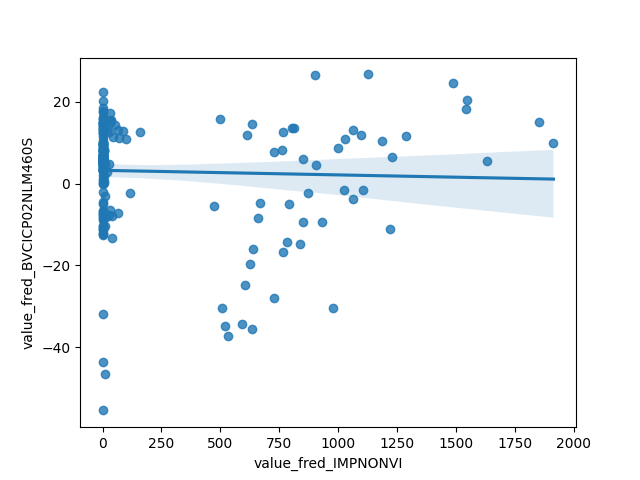
\includegraphics[scale = 0.9]{plots/plot_2026-09-03.png}
\caption{Raw Regression Plot for 2026-09-03}
\end{figure}
\newpage
\subsection{Detrended Regression}
\noindent Regresses the residuals of each series after removing its own linear time trend, so a shared trend can no longer drive the result on its own. A relationship that stays significant here is better evidence of a genuine link between the two series.

\begin{center}
\begin{tabular}{lclc}
\toprule
\textbf{Dep. Variable:}                   & value\_fred\_BVCICP02NLM460S\_detrended & \textbf{  R-squared:         } &     0.027   \\
\textbf{Model:}                           &                   OLS                   & \textbf{  Adj. R-squared:    } &     0.023   \\
\textbf{Method:}                          &              Least Squares              & \textbf{  F-statistic:       } &     6.159   \\
\textbf{Date:}                            &             Thu, 03 Sep 2026            & \textbf{  Prob (F-statistic):} &   0.0138    \\
\textbf{Time:}                            &                 15:18:46                & \textbf{  Log-Likelihood:    } &   -871.17   \\
\textbf{No. Observations:}                &                     222                 & \textbf{  AIC:               } &     1746.   \\
\textbf{Df Residuals:}                    &                     220                 & \textbf{  BIC:               } &     1753.   \\
\textbf{Df Model:}                        &                       1                 & \textbf{                     } &             \\
\textbf{Covariance Type:}                 &                nonrobust                & \textbf{                     } &             \\
\bottomrule
\end{tabular}
\begin{tabular}{lcccccc}
                                          & \textbf{coef} & \textbf{std err} & \textbf{t} & \textbf{P$> |$t$|$} & \textbf{[0.025} & \textbf{0.975]}  \\
\midrule
\textbf{const}                            &   -5.169e-13  &        0.826     & -6.26e-13  &         1.000        &       -1.627    &        1.627     \\
\textbf{value\_fred\_IMPNONVI\_detrended} &       0.0067  &        0.003     &     2.482  &         0.014        &        0.001    &        0.012     \\
\bottomrule
\end{tabular}
\begin{tabular}{lclc}
\textbf{Omnibus:}       & 85.354 & \textbf{  Durbin-Watson:     } &    0.157  \\
\textbf{Prob(Omnibus):} &  0.000 & \textbf{  Jarque-Bera (JB):  } &  284.269  \\
\textbf{Skew:}          & -1.608 & \textbf{  Prob(JB):          } & 1.87e-62  \\
\textbf{Kurtosis:}      &  7.515 & \textbf{  Cond. No.          } &     307.  \\
\bottomrule
\end{tabular}
%\caption{OLS Regression Results}
\end{center}

Notes: \newline
 [1] Standard Errors assume that the covariance matrix of the errors is correctly specified.

\begin{figure}
\centering
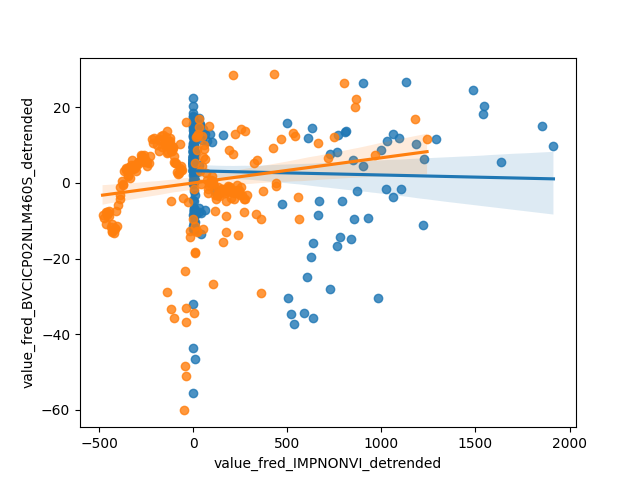
\includegraphics[scale = 0.9]{plots/plot_2026-09-03_detrended.png}
\caption{Detrended Regression Plot for 2026-09-03}
\end{figure}
\newpage
